\chapter{Revisiting a Randomness Beacon Protocol}
\label{cha:n}

Randomness Beacon \cite{RABIN1983256} is required in applications like e-voting \cite{10.5555/1496711.1496734} 
and anonymous messaging (\cite{180263},\cite{10.1145/2815400.2815417}) to provide fresh unbiased random values to all the 
parties. In 2020, Cascudo and David published ALBATROSS \cite{cryptoeprint:2020/644}, the state-of-the art randomness 
beacon protocol based on a PVSS as a building block where each party in the randomness beacon protocol acts as a dealer once, so that all 
parties can influence the output randomness. Interestingly, we observed that each party is expected to reveal 
their secrets (they secret shared as a dealer) as part of the randomness beacon protocol, but to prove that the 
secrets are valid and not just some random evaluations of the secret polynomial, they have to reveal the whole 
secret polynomial itself. As a consequence, if some entity wants to verify the secrets' validity then they have to 
simulate the whole sharing phase of the underlying PVSS protocol, which is very expensive because all the rest of the 
parties are expected to do the simulation of that party as a dealer. For reference, if there are $n$ parties, then 
$n-1$ parties should simulate the sharing phase of the protocol, which in total is $\mathcal{O}(n^2)$ simulations.\par

In this chapter, we present our randomness beacon protocol in figures \ref{fig:randomness_beacon} and \ref{fig:randomness_beacon_cont} 
which in many cases is efficient than ALBATROSS. To put simply, we replaced the building block being PVSS with 
our 3PVSS $\Lambda_{RO}^{packed}$ \ref{fig:packed-shamir-PPPVSS-ro}. In the subsequent sections, we will discuss a 
bottleneck in ALBATROSS protocol, security 
analysis of our protocol briefly, followed by the 
computational and communication costs of our protocol and compare it with the ALBATROSS. We will show that our protocol 
performs more efficiently when compared to ALBATROSS in many cases and also address the cases where we are not computationally efficient.
More interestingly, we will show that in terms of communication, we outperform ALBATROSS.

\begin{figure}[ht]
    \centering
    \begin{tcolorbox}[title=\textbf{Randomness Beacon using PPPVSS}, width=0.9\textwidth, colframe=blue!75!black, colback=blue!10, sharp corners]
        Our protocol with PPPVSS is run between a set $\mathcal{P}$ of $n$ 
        parties $P_1, \dots, P_n$ who have access to a public ledger where they 
        can post information for later verification. It is assumed that the 
        Setup phase of $\Pi_{PPPVSS}$ is already done and the public keys 
        $\text{pk}_i$ of each party $P_i$ along with $\{\mathbb{P}_i\}_{i=1}^{l}$ 
        being Commitment keys (or public keys of target people) to encrypt the 
        $l$ secrets are already registered in the ledger. In addition, the 
        parties have agreed on a Vandermonde $(n - 2t) \times (n - t)$-matrix 
        $M = M(\omega, n - 2t, n - t)$ with $\omega \in \mathbb{Z}_q^*$.

    \begin{enumerate}
        \item [1.]\textbf{Commit:} For $1 \leq j \leq n$:
        \begin{itemize}
            \item Shareholder $P_j$ executes the Distribution phase of the 
            PPPVSS as Dealer for $\ell = n - 2t$ secrets, publishing commitments 
            (/encryptions) of secrets, $y_{-(l-1)}^j, \dots, y_{-1}^j, y_0^j$, 
            and encryptions of shares $\{y_i^j\}_{i=1}^n$ along with 
            $\pi_{proof}^{j}$, which is a NIZK PoK for proving the correctness of 
            committed(/encrypted) secrets and encrypted secret shares on the 
            public ledger, also learning the secrets $h^{s_0^j},...,h^{s_{-(l-1)}^j}$ 
            and their corresponding exponents\\ $s_0^j, \dots, s_{-(l-1)}^j$.
        \end{itemize}
        
        \item [2.]\textbf{Reveal:}
        \begin{itemize}
            \item Each shareholder checks the validity of the proof 
            $\pi_{proof}^j$, i.e., the \textbf{verification phase of PPPVSS protocol}.
            \item After a set $\mathcal{C}$ containing at least $n-t$ 
            shareholders publish their shares in the public ledger, 
            $P_j\in\mathcal{C}$ reveals $l$ secrets.
            \item Every shareholder verifies the validity of secrets by 
            reproducing the commitments using the commitment keys (/public keys 
            of target people).
            \item At this point, if every party in $\mathcal{C}$ has opened 
            their secrets correctly, go to step 4' in Figure \ref{fig:9}. 
            Otherwise, proceed to step 3 in Figure \ref{fig:9}.
        \end{itemize}
    \end{enumerate}
    \end{tcolorbox}
    \caption{Commit and Reveal phase of the Randomness Beacon using PPPVSS}
    \label{fig:randomness_beacon}
\end{figure}
\begin{figure}[t!]
    \centering
    \begin{tcolorbox}[title=\textbf{Randomness Beacon using 3PVSS, $\Lambda_{RO}^{packed}$ (cont.)}, width=0.9\textwidth, colframe=blue!75!black, colback=blue!10, sharp corners]
        \begin{enumerate}
            \item [3.]\textbf{Recovery:} Let $\mathcal{C}_a$ be the set containing at most $t$ malicious shareholders(as Dealers) who did not open the exponents corresponding to their $\ell$ secrets, $\{h^{s_i^k}\}_{i=0}^{-(\ell-1)}$ for each $P_k\in\mathcal{C}_a$, in \textit{Reveal} phase.
            \begin{itemize}
                \item Every shareholder $P_j$ should decrypt the secret share of each malicious shareholder(Dealer) in $\mathcal{C}_a$, and give a DLEQ proof \ref{subsec:chaum-pedersen} which asserts that the decryption is performed correctly,i.e., each shareholder should perform the \textit{pessimistic} reconstruction phase of the 3PVSS $\Lambda_{RO}^{packed}$ for every shareholder(Dealer) who has not revealed the exponents corresponding to their secrets.
            \end{itemize}
            
            \item [4]\textbf{Output:}  Let $T$ be the $(n - t) \times \ell$ matrix with rows indexed by the shareholders in $\mathcal{C}$ and where the row corresponding to $P_a \in \mathcal{C}$ is $(h^{s_0^a} , . . . , h^{s_{-(\ell-1)}^a})$.
            \begin{itemize}
                \item Each computes the $\ell \times \ell$-matrix $R = M \circ T$ by applying FFTE to each column $T^{(j)}$ of $T$, resulting in column $R^{(j)}$ of $R$ (since $R^{(j)} = M \circ T^{(j)}$ and $M$ is Vandermonde) for $j \in [0, \ell - 1]$.
                \item Shareholders output the $\ell^2$ elements of $R$ as final randomness.
            \end{itemize}
        
            \item [4']\textbf{Alternative Output:}  if every party in $\mathcal{C}$ has opened her secrets correctly in step \textit{Reveal}, then:
            \begin{itemize}
                \item Shareholders compute $R = M \circ T$ in the following way:\\
                    Let $S$ be the $(n - t) \times \ell$ matrix with rows indexed by the shareholders in $\mathcal{C}$ and where the row
                    corresponding to $P_a \in\mathcal{C}$ is $(s_0^a,...,s_{-(\ell-1)}^a )$. Then each party computes $U = M \circ S \in\mathbb{Z}_q^{\ell\times \ell}$ (using the standard FFT in $\mathbb{Z}_q$ to compute each column) and $R = h^U$ .
                \item Shareholders output the $\ell^2$ elements of $R$ as final randomness.
            \end{itemize}
        \end{enumerate}
    \end{tcolorbox}
    \caption{Recovery and Output phase of the Randomness Beacon using 3PVSS}
    \label{fig:randomness_beacon_cont}
\end{figure}

\section{On the bottleneck of ALBATROSS}
The main bottleneck of ALBATROSS is in its \textit{Reveal} phase (description in 
figure 8 in section 4.3 of \cite{cryptoeprint:2020/644}). More precisely, the 
goal of the \textit{Reveal} phase is to reveal the secrets of whom the dealer has done the 
secret sharing. But in order to verify that those values are actual secrets, in ALBATROSS, a 
verifier has to simulate the whole sharing phase of the dealer with the values that were 
revealed. This is because, the underlying proof system of a general PVSS says that \textit{if the 
PVSS verification algorithm outputs true, then the encryptions of the secret shares correspond 
to some unique secret with high probability}.\par

Whereas, in the case of (P)PPVSS, \textit{if the verification algorithm outputs true then it means 
that the encryptions of the secret shares correspond to the unique secret(s) which was 
already committed by the dealer (which is the reason why commitment value of secret(s) 
is a part of the proof statement) with high probability}. So, the intuition is that if one 
uses a PPVSS, that packs multiple secrets in a single polynomial, over the PVSS used in 
ALBATROSS (a Random Beacon protocol) then the efficiency of the new Randomness beacon 
protocol can be improved.

\section{Security analysis}
This section will briefly discuss why our protocol can remain secure. Note that, the major changes 
in our protocol in contrast to ALBATROSS are the \textit{Commit} and \textit{Reveal} 
phases. As long as the randomizers used to commit (/secret keys to decrypt) secrets are 
not leaked then \textit{Commit} phase is as secure such that it does not reveal anything 
about the secrets. This is because of the mathematical security guarantees achieved 
through the sharing phase of our 3PVSS, $\Lambda_{RO}^{packed}$.\par

In ALBATROSS, the whole point of the \textit{Reveal} phase is to open the secrets itself, 
but to verify that the secrets are valid for a given secret shares, one has to simulate 
the whole sharing phase of the respective dealer. As our 3PVSS, $\Lambda_{RO}$, already 
proves that the commitment is a valid commitment of dealers' secrets and their respective 
secret sharing is done correctly, it does not require to perform the whole simulation of 
the sharing phase of any dealer. Because the dealer has already committed to the 
secrets, he cannot cheat by revealing wrong secrets. Therefore, the \textit{Reveal} 
phase of our protocol also is secure due to the security guarentees of $\Lambda_{RO}^{packed}$.

\section{Computational Complexity}
\begin{table}[H]
\centering
\begin{tabular}{|p{3cm}|p{1.2cm}|p{2.5cm}|p{5.5cm}|p{2.5cm}|}
\hline
\textbf{Protocol}    & \textbf{Output size}    & 
\textbf{Commit}\textit{(by Dealer)} & \textbf{Reveal}\textit{(by 
shareholder)} & \textbf{Recovery} \textit{(by shareholder)}                                                           
\\ \hline
\textbf{ALBATROSS}, \textit{Honest case}    & $l^2$ & 
$(2n+l)[\mathbb{E}_x+\mathbb{P}_e]$ & \textbf{Share Verification - }  &  
\\
& & & $(n-1)n[2\mathbb{E}_x+\mathbb{P}_e]$ & \\
& & & \textbf{Secret Verification - } & \\ 
& & & $(n-1)(n+l)[\mathbb{E}_x+\mathbb{P}_e]$&- \\ \hline
\textbf{with PPPVSS}, \textit{Honest case}    & $l^2$  & 
$2(n+l)[\mathbb{E}_x+\mathbb{P}_e]$ & \textbf{Share Verification - } &  \\ 
& & & $(n-1)(n+l)[2\mathbb{E}_x+\mathbb{P}_e]$ &  \\ 
& & & &  \\
& & & \textbf{Secret Verification - } & \\ 
& & & $(n-1)l\mathbb{E}_x$ & -  \\ \hline
\textbf{ALBATROSS}, \textit{Robust case}    & $l^2$ & 
$(2n+l)[\mathbb{E}_x+\mathbb{P}_e]$ & \textbf{Share Verification - }  &  
\\
& & & $(n-1)n[2\mathbb{E}_x+\mathbb{P}_e]$ & \\
& & & \textbf{Secret Verification - } & \\ 
& & & $(n-t-1)(n+l)[\mathbb{E}_x+\mathbb{P}_e]$& 
$[3+4(n-t)]t\mathbb{E}_{x}$\\ \hline
\textbf{with PPPVSS}, \textit{Robust case}    & $l^2$  & 
$2(n+l)[\mathbb{E}_x+\mathbb{P}_e]$ & \textbf{Share Verification - } &  \\ 
& & & $(n-1)(n+l)[2\mathbb{E}_x+\mathbb{P}_e]$ &  \\
& & & \textbf{Secret Verification - } & \\ 
& & & $(n-t-1)l\mathbb{E}_x$ &   \\
& & & & $[3+4(n-t)]t\mathbb{E}_{x}$  \\ \hline

\end{tabular}
\caption{Computational cost of dealer and shareholders, 
$\mathbb{E}_x=$group exponentiation and $\mathbb{P}_e=$polynomial 
evaluation in group $G$ with order $q$, where $q$ is a large prime}
\label{tab:comp_alba_pppvss_no group mul}
\end{table}


One would notice that the major changes are in the commit and reveal phase of the protocol. 
Hence, in this section we only will talk about the performance analysis in those 
phases. See table \ref{tab:comp_alba_pppvss_no group mul} for an overview. Also, we ignore the number of 
multiplications in the group $\mathbb{G}$, i.e., $M_{\mathbb{G}}$ in the table as it is negligible compared to 
the number of group exponentiations $\mathbb{E}_x$ with random exponents in practice. 
\begin{itemize}
    \item In ALBATROSS, a dealer(as a part of \textbf{commit}) should compute $n(\mathbb{E}_x+\mathbb{P}_e)$ commitments and to give a proof he should do an additional $n(\mathbb{E}_{x}+\mathbb{P}_e)$. Also, the dealer should do $\ell(\mathbb{E}_x+\mathbb{P}_e)$ for computing secrets and keeping it to himself. In total dealer needs to do $(2n+\ell)[\mathbb{E}_x+\mathbb{P}_e]$.
        \begin{itemize}
            \item In \textbf{Reveal}, a verifier should compute $2n\mathbb{E}_{x}$ which internally requires additional $n\mathbb{P}_e$, i.e., in total it requires $(n-1)n(2\mathbb{E}_{x}+\mathbb{P}_{e})$ computations for each verifier.
            \begin{itemize}
                \item In \textbf{Robust case} where $t$ dealers do not open their polynomials, a verifier should verify $n-t$ polynomials of honest dealers, i.e., for each honest dealer, a verifier has to do $n\mathbb{P}_e$ to evaluate secret share exponents and does $n\mathbb{E}_x$ to get secret shares and cross checks them in the public ledger. Also, finally the verifier computes $\ell\mathbb{P}_e$ to get secret exponents and get $\ell$ secrets by doing $\ell\mathbb{E}_x$. As there are $n-t$ honest dealers, the verifier has to compute $(n-t)(n+\ell)(\mathbb{E}_x+\mathbb{P}_e)$.
                \item  In \textbf{Honest case}, everyone would have been honest and so each verifier has to do $(n-1)(n+\ell)(\mathbb{E}_x+\mathbb{P}_e)$.
            \end{itemize}
            \item \textbf{Recovery} phase only exists if some party does not 
            open the polynomial leading to PVSS reconstruction phase, in the 
            worst case there should be reconstruction for the secrets of $t$ 
            malicious parties. Given a malicious shareholder who has not opened 
            the secret polynomial, each shareholder/re-constructor has to 
            decrypt their share, which requires $1\mathbb{E}_{x}$ and should 
            give a DLEQ proof that they have decrypted correctly, which 
            additionally requires $2\mathbb{E}_x$; Also the re-constructor 
            should verify DLEQ proofs of correct share decryption from $n-t$ 
            honest shareholders requiring them to do $4(n-t)\mathbb{E}_{x}$. 
            In total, each re-constructor requires $[3+4(n-t)]t\mathbb{E}_{x}$.
        \end{itemize}
    \item Using 3PVSS in randomness beacon protocol, a dealer(as a part of \textbf{commit}) requires to do $(n+\ell)[\mathbb{E}_x+\mathbb{P}_e]$ and $(\ell-1)M_\mathbb{G}$ to compute $\{y_i\}_{i=0}^{n}$. For generating the proof that $y_i$'s are valid encryptions of the secret shares and also $y_0$ is a commitment of the $\ell$ secrets, the dealer should do $(n+\ell)[\mathbb{E}_x+\mathbb{P}_e]$ which internally requires additional $(\ell-1)M_\mathbb{G}$. In total, a dealer has to do $2\left[(n+\ell)[\mathbb{E}_x+\mathbb{P}_e]+(\ell-1)M_\mathbb{G}\right]$.
    \begin{itemize}
        \item In \textbf{Reveal}, a verifier should do $(n+\ell)(2\mathbb{E}_x+\mathbb{P}_e)$ and $(\ell-1)M_\mathbb{G}$ for each proof. In total, a verifier has to do $(n-1)(n+\ell)[2\mathbb{E}_x+\mathbb{P}_e]+(n-1)(\ell-1)M_\mathbb{G}$.
        \begin{itemize}
            \item In \textbf{Robust case} with $t$ malicious parties not opening the secret polynomials, a verifier should do $\ell\mathbb{E}_x+(\ell-1)M_\mathbb{G}$ to verify each proof, so in total each verifier should do $(n-t-1)[l\mathbb{E}_x+(\ell-1)M_\mathbb{G}]$.
            \item In \textbf{Honest case} where everyone is honest, a verifier will do $(n-1)\ell(\mathbb{E}_x+M_\mathbb{G})$.
        \end{itemize}
        \item The computational complexity of each re-constructor in \textbf{Recovery} phase is exactly same as in the case of ALBATROSS.
    \end{itemize}
\end{itemize}

\subsection{Computational Cost analysis}
The dealer has to do a bit more work in the case of our protocol in contrast to ALBATROSS, more explicitly, 
they have to compute $\ell$ more group exponentiations and polynomial evaluations. But as a consequence, 
we decrease computational cost in the \textit{Reveal} phase whenever $\ell < \frac{n(n-t-1)}{2(n-1)}$, roughly 
speaking, if the number of secrets are less than half of the honest parties then we always perform better in 
terms of computation when compared to the ALBATROSS.\par

More precisely, in the reveal phase, we observed that our protocol gains at least $30\%$ more
efficiency for performing polynomial evaluations, and at least $23\%$ more efficiency for 
performing group exponentiations when compared to ALBATROSS in the robust case where the number of 
secrets $\ell$ is equal to one. See plots \ref{fig:commit_polynomial} 
and \ref{fig:commit_exponent} for the performance analysis of polynomial evaluations and group exponentiations
in the reveal phase of our protocol and ALBATROSS.

\begin{figure}[htbp]
  \centering
  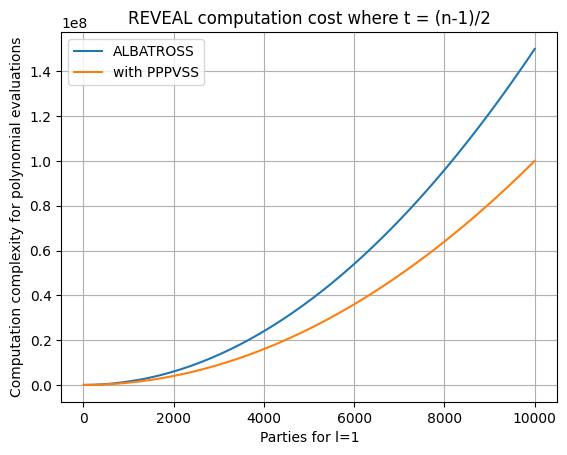
\includegraphics[width=0.7\textwidth]{figures/polynomial.png}
  \caption{Your caption here}
  \label{fig:your-label}
\end{figure}
\begin{figure}[htbp]
  \centering
  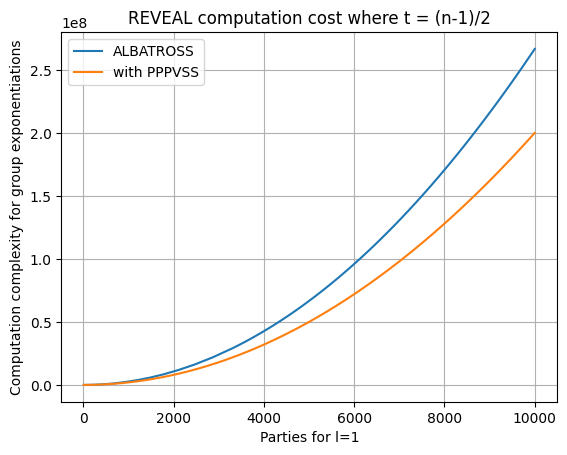
\includegraphics[width=0.7\textwidth]{figures/exponent.png}
  \caption{Your caption here}
  \label{fig:commit_exponent}
\end{figure}

\section{Communication Complexity}
\begin{table}[H]
\centering
\begin{tabular}{|p{3cm}|p{4cm}|p{3.5cm}|p{4cm}|p{1cm}|}
\hline
\textbf{Protocol}     & \textbf{Commit} \textit{(by Dealer)} & \textbf{Reveal} \textit{(by Dealer)} & \textbf{Recovery}  \textit{(by shareholder)}                                                      \\ \hline
\textbf{ALBATROSS}   & $nG+(t+l)\mathbb{Z}_q$ & $(t+l)\mathbb{Z}_q$ & $1G+1\mathbb{Z}_q+1R_o$ \\ \hline
\textbf{with PPPVSS}    & $(n+1)G+(t+l)\mathbb{Z}_q$ & $l\mathbb{Z}_q$ & $1G+1\mathbb{Z}_q+1R_o$ \\ \hline

\end{tabular}
\caption{Communication cost of dealer and (each) shareholder, $R_o$ being the random oracle, $G = $group of order $q$ and $\mathbb{Z}_q =$ modular group of order $q$, where $q$ is a large prime}
\label{tab:dealer_comm}
\end{table}

See table \ref{tab:dealer_comm} for an overview.
\begin{itemize}
    \item In ALBATROSS, a dealer (as a part of \textbf{commit}) should send $n$ group elements as commitments, $t+\ell$ elements in $\mathbb{Z}/q\mathbb{Z}$ that defines the polynomial used in the ZKP and $1$ extra element in $\mathbb{Z}/q\mathbb{Z}$ from RO. 
    \begin{itemize}
        \item In \textbf{Reveal}, an honest dealer would broadcast $t+\ell$ coefficients in $\mathbb{Z}/q\mathbb{Z}$ concerning the secret polynomial.
        \item If some party has not revealed their polynomial, then in \textbf{Recovery} phase a re-constructor using PVSS reconstruction protocol should broadcast $1$ element in group which is being the decrypted secret, for the proof of correct decryption, they have to broadcast $3$ more group elements along with a polynomial which requires $t+\ell$ coefficients in $\mathbb{Z}/q\mathbb{Z}$ and $1$ group element from RO.
    \end{itemize}
    \item Using 3PVSS in randomness beacon protocol, a dealer (as a part of \textbf{commit}) should send $n+1$ group elements as commitments, $t+\ell$ elements in $\mathbb{Z}/q\mathbb{Z}$ that defines the polynomial used in the ZKP and $1$ extra element in $\mathbb{Z}/q\mathbb{Z}$ from RO.
    \begin{itemize}
        \item In \textbf{Reveal}, an honest dealer would broadcast $\ell$ elements in $\mathbb{Z}_q$ concerning the exponents to construct the secret.
        \item If some part has not revealed their secrets, then the communication cost of each re-constructor is exactly same as in the case of ALBATROSS.
    \end{itemize}
\end{itemize}

\subsection{Communication Cost analysis}
The best to offer from our randomness beacon protocol is the communication cost. Though the dealer has to communicate only 
one extra group element compared to ALBATROSS in the commit phase, as a consequence for a fixed number of secrets the 
dealers' communication cost is constant as opposed to linear in number of corrupted parties in ALBATROSS. \par

In the plots \ref{fig:dealer_commit_comm} and \ref{fig:comm_reveal}, we show the communication cost of a dealer to bare 
in ALBATROSS and our protocol in both the commit and reveal phases.

\begin{figure}[H]
  \centering
  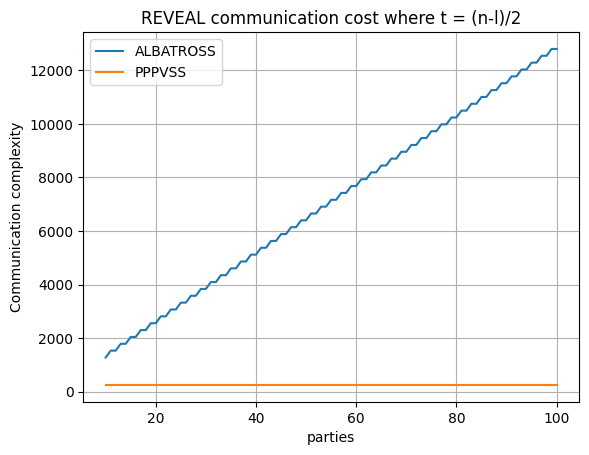
\includegraphics[width=0.7\textwidth]{figures/reveal_comm.png}
  \caption{Communication cost of a dealer in reveal phase of ALBATROSS and our protocol}
  \label{fig:comm_reveal}
\end{figure}

\begin{figure}[htbp]
  \centering
  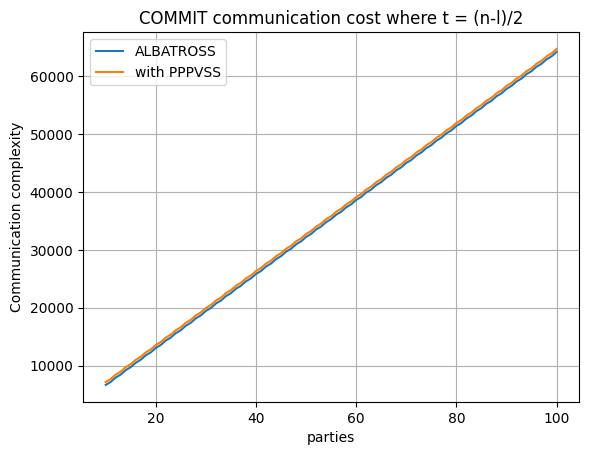
\includegraphics[width=0.7\textwidth]{figures/commit_comm.png}
  \caption{Your caption here}
  \label{fig:dealer_commit_comm}
\end{figure}

%%% Local Variables: 
%%% mode: latex
%%% TeX-master: "thesis"
%%% End: 
